\documentclass[18pt,aspectratio=149]{beamer}
\usepackage[]{bookmark}
\usepackage[utf8]{inputenc}
\usepackage{amsmath}
\usepackage{amsfonts}
\usepackage{amssymb}
\usepackage{tikz}
\usepackage{xcolor}
\usepackage{sansmathaccent}
\usepackage{graphicx}

\usepackage[style=alphabetic,backend=biber]{biblatex} 
\addbibresource{bibliography.bib}

\addbibresource{bibliography.bib} 
\pdfmapfile{+sansmathaccent.map}

\title{The use/abuse of copulas in actuarial science and finance}
\author{Isidoor Pinillo Esquivel}
\usetheme{Madrid}
\date{}

\begin{document}

\begin{frame}
    \titlepage
\end{frame}
\begin{frame}
    \frametitle{Overview}
    \begin{itemize}
        \item Literature overview
        \item Modelling dependence
        \item Copulas
        \item Tools
        \item Conclusion
    \end{itemize}
\end{frame}

\begin{frame}
    \frametitle{Papers}
    \begin{itemize}
        \item \citetitle{dempster_correlation_2002},\\ \textcite{dempster_correlation_2002}
        \item \citetitle{frees_understanding_1998},\\ \textcite{frees_understanding_1998}
        \item \citetitle{donnelly_devil_nodate},\\ \textcite{donnelly_devil_nodate}
        \item \citetitle{lopez-paz_dependence_2016},\\ \textcite{lopez-paz_dependence_2016}
    \end{itemize}

\end{frame}

\begin{frame}
    \frametitle{Favorite course on yt with a section on dependence}
    \begin{center}
        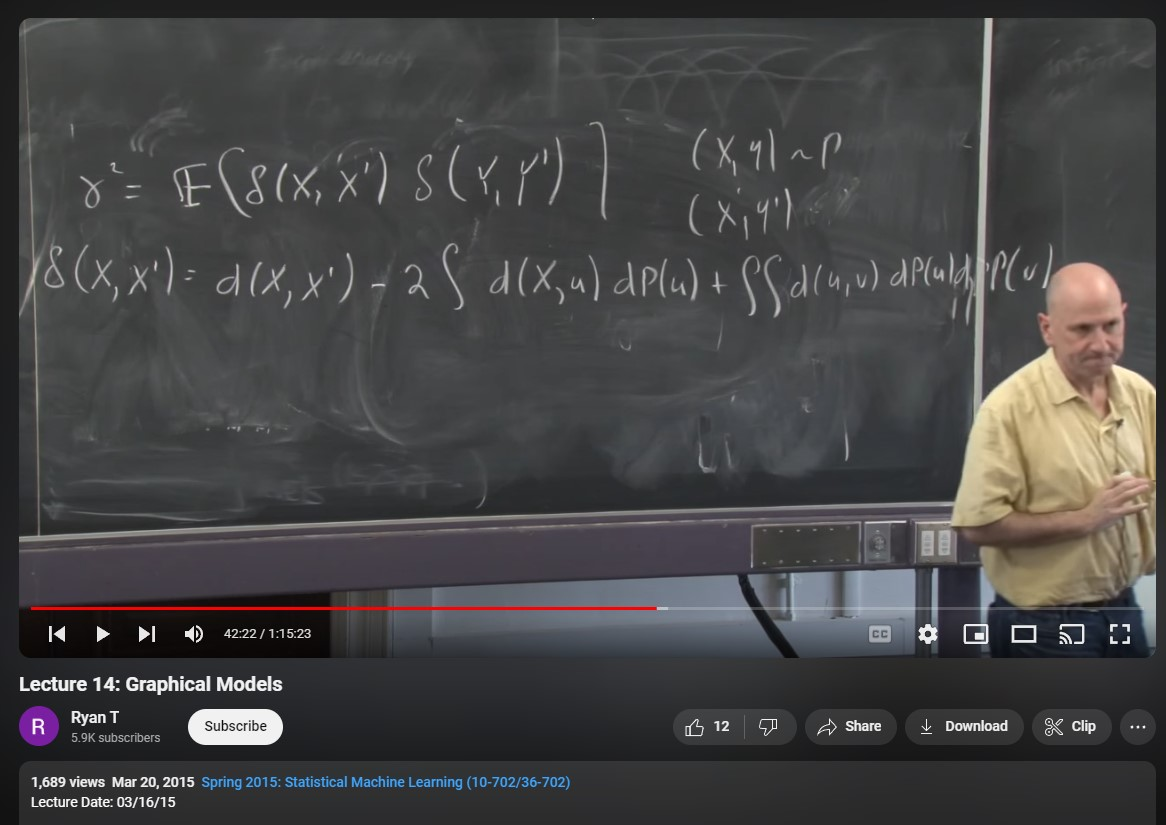
\includegraphics[width=0.7\textwidth]{graphical models yt.jpg}
    \end{center}
\end{frame}

\begin{frame}
    \frametitle{Dependence}
    \begin{center}
        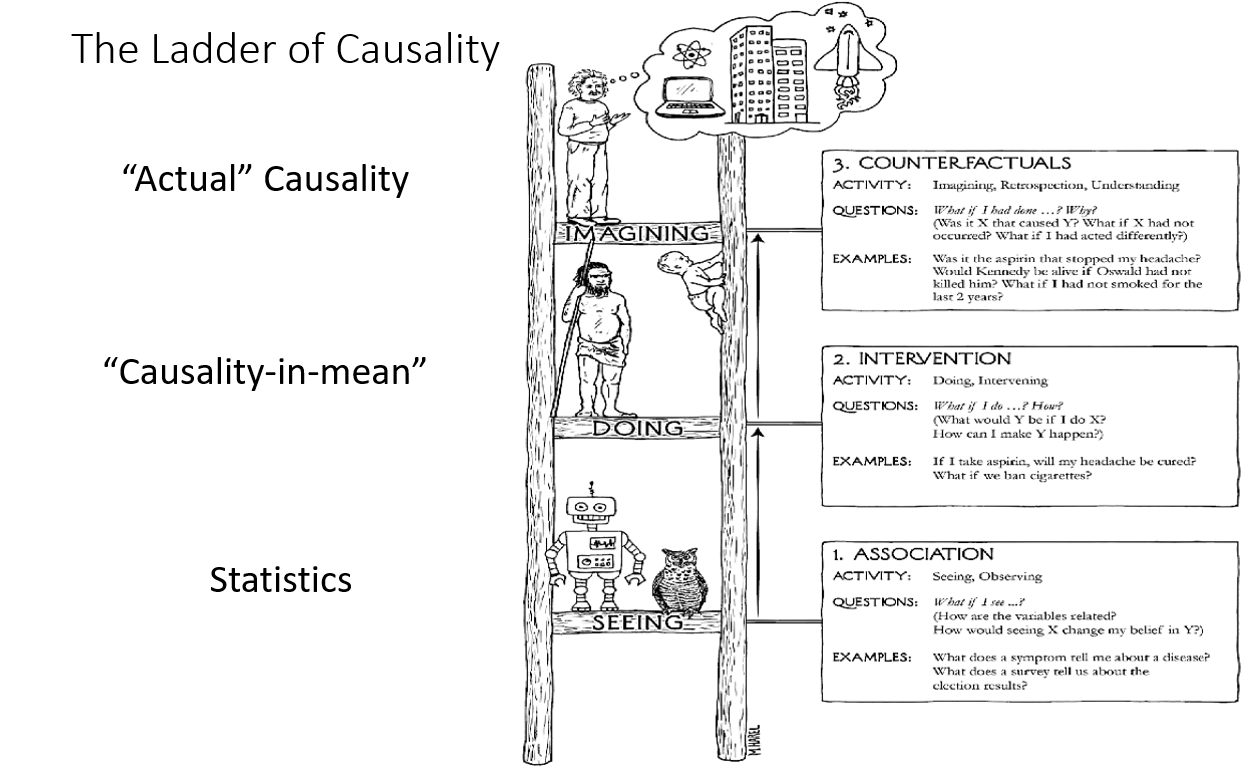
\includegraphics[width=0.8\textwidth]{Ladder-1.png}
    \end{center}
\end{frame}

\begin{frame}
    \frametitle{Modelling dependence $1$}
    \begin{itemize}
        \item Modelling with multivariate RVs $\rightarrow$ density estimation
        \item Usually only data and domain knowledge
        \item Non-parametric vs parametric
        \item Data and computational limitations
        \item Approximate assumptions
        \item Issues at tails
        \item Marginals + copulas
    \end{itemize}
\end{frame}



\begin{frame}
    \frametitle{Multivariate CLT}
    \begin{center}
        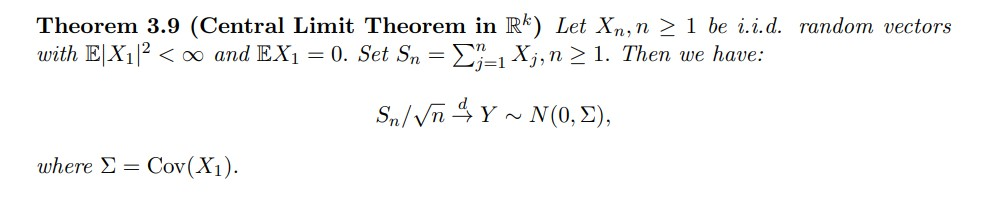
\includegraphics[width=0.9\textwidth]{CLT.jpg}
        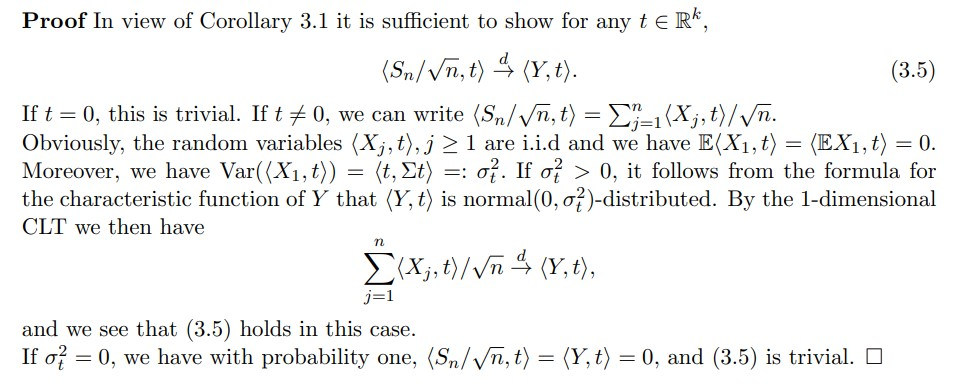
\includegraphics[width=0.9\textwidth]{CLT2.jpg}
    \end{center}
\end{frame}

\begin{frame}
    \frametitle{Gaussian copula}
    Sklar's theorem $\rightarrow$ transform the marginals to uniforms \\
    Same amount parameters as the Gaussian distribution \\
    No parametric assumption on marginals compared to assuming Gaussian

    \begin{center}
        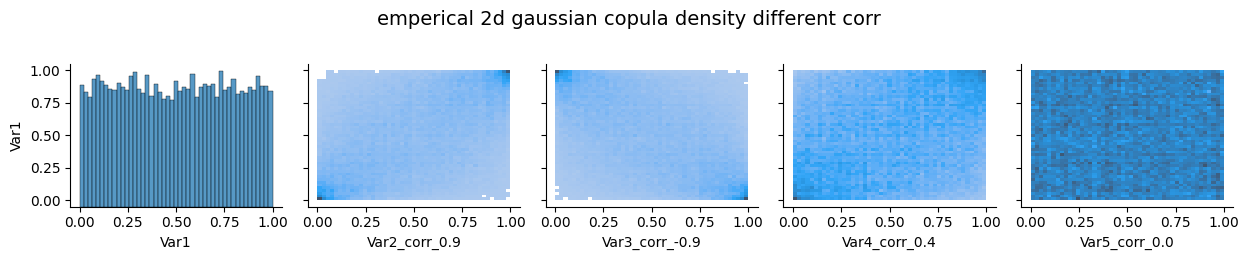
\includegraphics[width=\textwidth]{gaussian_copula.png}
    \end{center}

\end{frame}


\begin{frame}
    \frametitle{Spherical/elliptical distributions 1}
    Spherical distributions have a spherical/elliptical symmetry or\\
    \begin{equation}
        X =_{d} R U
        .
    \end{equation}
    with $R>0,U\perp\!\!\!\perp R$ uniform on unit sphere. \\
    \pause

    Elliptical distributions $=$ affine transformations of spherical distributions. \\
    \pause
    Parametrized by mean, covariance matrix and $R$. \\
    Semi-parametric multivariate distributions
\end{frame}

\begin{frame}
    \frametitle{Spherical/elliptical distributions 2}
    The intersection between ellipsoids and planes are also ellipsoids similar:
    \pause
    \begin{itemize}
        \item An affine transformation of an elliptical distribution is also elliptical.
        \item The sum in the set of elliptical distributions with the same generator is closed.
        \item Marginal and conditional  distributions of the components of elliptical distributions are elliptical.
    \end{itemize}
    \pause
    \vspace{0.5cm}
    In \cite{dempster_correlation_2002} they show that linear portfolios where individual risk together are jointly elliptical
    distributed, \textbf{risk measures lose structure}, simplifying risk management tasks. Specifically they show that VaR is equivalent
    to variance risk analysis.
\end{frame}

\begin{frame}
    \frametitle{Tail dependence 1}
    Tail dependence $\approx$ dependence in the tails .
    The upper tail dependence ($\lambda$) between $X$ and $Y$ is defined as follows:
    \begin{equation}
        \lim_{\alpha \to 1-}  P[ Y > F_{Y}^{-1} ( \alpha)
                \mid X > F_{X}^{-1} ( \alpha) ]=\lambda.
    \end{equation}
    \pause

    \cite{dempster_correlation_2002} show different ways to calculate tail dependence. They show
    that normal distributions have no tail dependence.
\end{frame}

\begin{frame}
    \frametitle{Tail dependence 2}
    When $X$ and $Y$ are continuous distribution we can express this in terms
    of their copula:
    \vspace{-0.5cm}
    {\small
        \begin{align}
             & \lim_{\alpha \to 1-}  P[ Y > F_{Y}^{-1} ( \alpha) \mid X > F_{X}^{-1} ( \alpha) ]                                          \\
             & =\lim_{\alpha \to 1-}  P[ U_{2} >  \alpha \mid U_{1} >  \alpha ]                                                           \\
             & =\lim_{\alpha \to 1-}  \frac{P[U_{1}>\alpha,U_{2}>\alpha]}{P[U_{1}>\alpha]}                                                \\
             & =\lim_{\alpha \to 1-}  \frac{1 - P[(U_{1}>\alpha,U_{2}>\alpha)^{c}]}{1-\alpha}                                             \\
             & =\lim_{\alpha \to 1-}  \frac{1 - P[(U_{1}\le \alpha) \cup ( U_{2}\le\alpha)]}{1-\alpha}                                    \\
             & =\lim_{\alpha \to 1-}  \frac{1 - P[U_{1}\le \alpha] - P[U_{2}\le \alpha]  + P[U_{1}\le \alpha , U_{2}\le\alpha]}{1-\alpha} \\
             & =\lim_{\alpha\to1-} \frac{1-2 \alpha +C(\alpha,\alpha)} {1-\alpha}.
        \end{align}
    }

\end{frame}

\begin{frame}
    \frametitle{Modelling CDOs}
    \begin{center}
        \begin{tikzpicture}
            \node[anchor=south west,inner sep=0] (image) at (0,0) {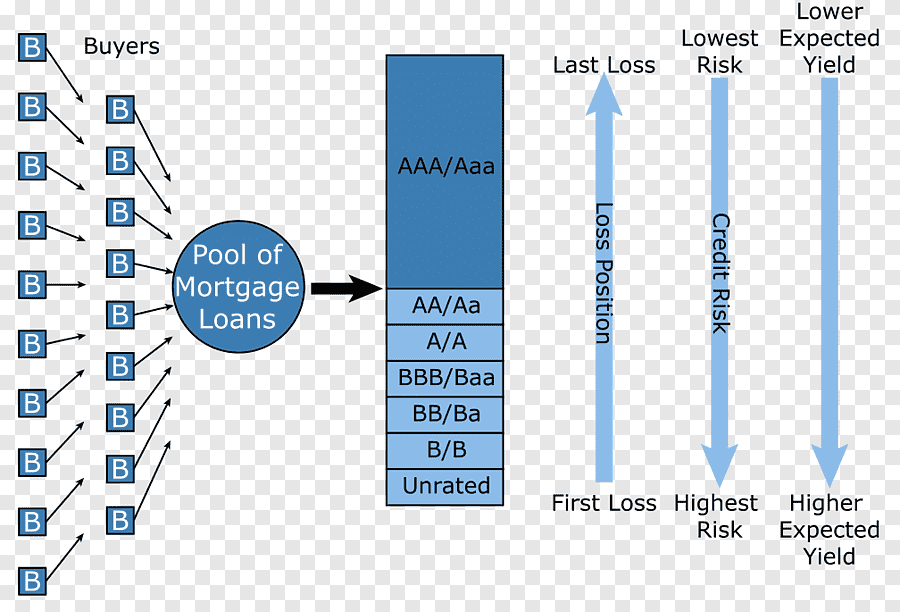
\includegraphics[width=0.7\textwidth]{cdo_ picture.png}};
            \pause
            \draw[<-, thick, red, shorten >=5pt] (10,5.5) -- (10,1) node[above, pos=0] {\scriptsize Modelling Risk};
        \end{tikzpicture}
    \end{center}
\end{frame}

\begin{frame}
    \frametitle{Visualizing with copulas $1$}
    \begin{center}
        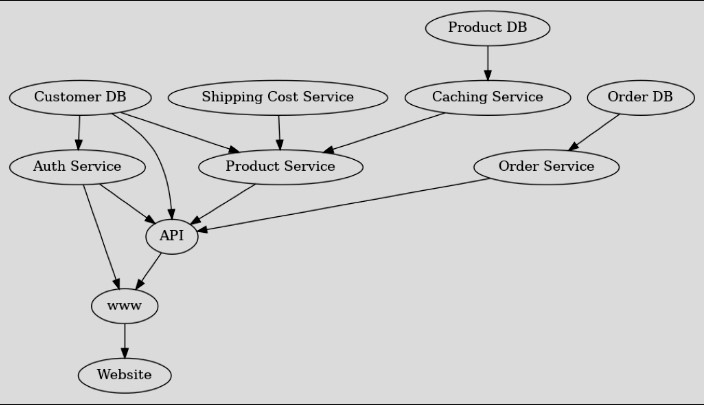
\includegraphics[width=0.9\textwidth]{microservice_structurejpg.jpg}
    \end{center}
\end{frame}

\begin{frame}
    \frametitle{Visualizing with copulas $2$}
    \begin{center}
        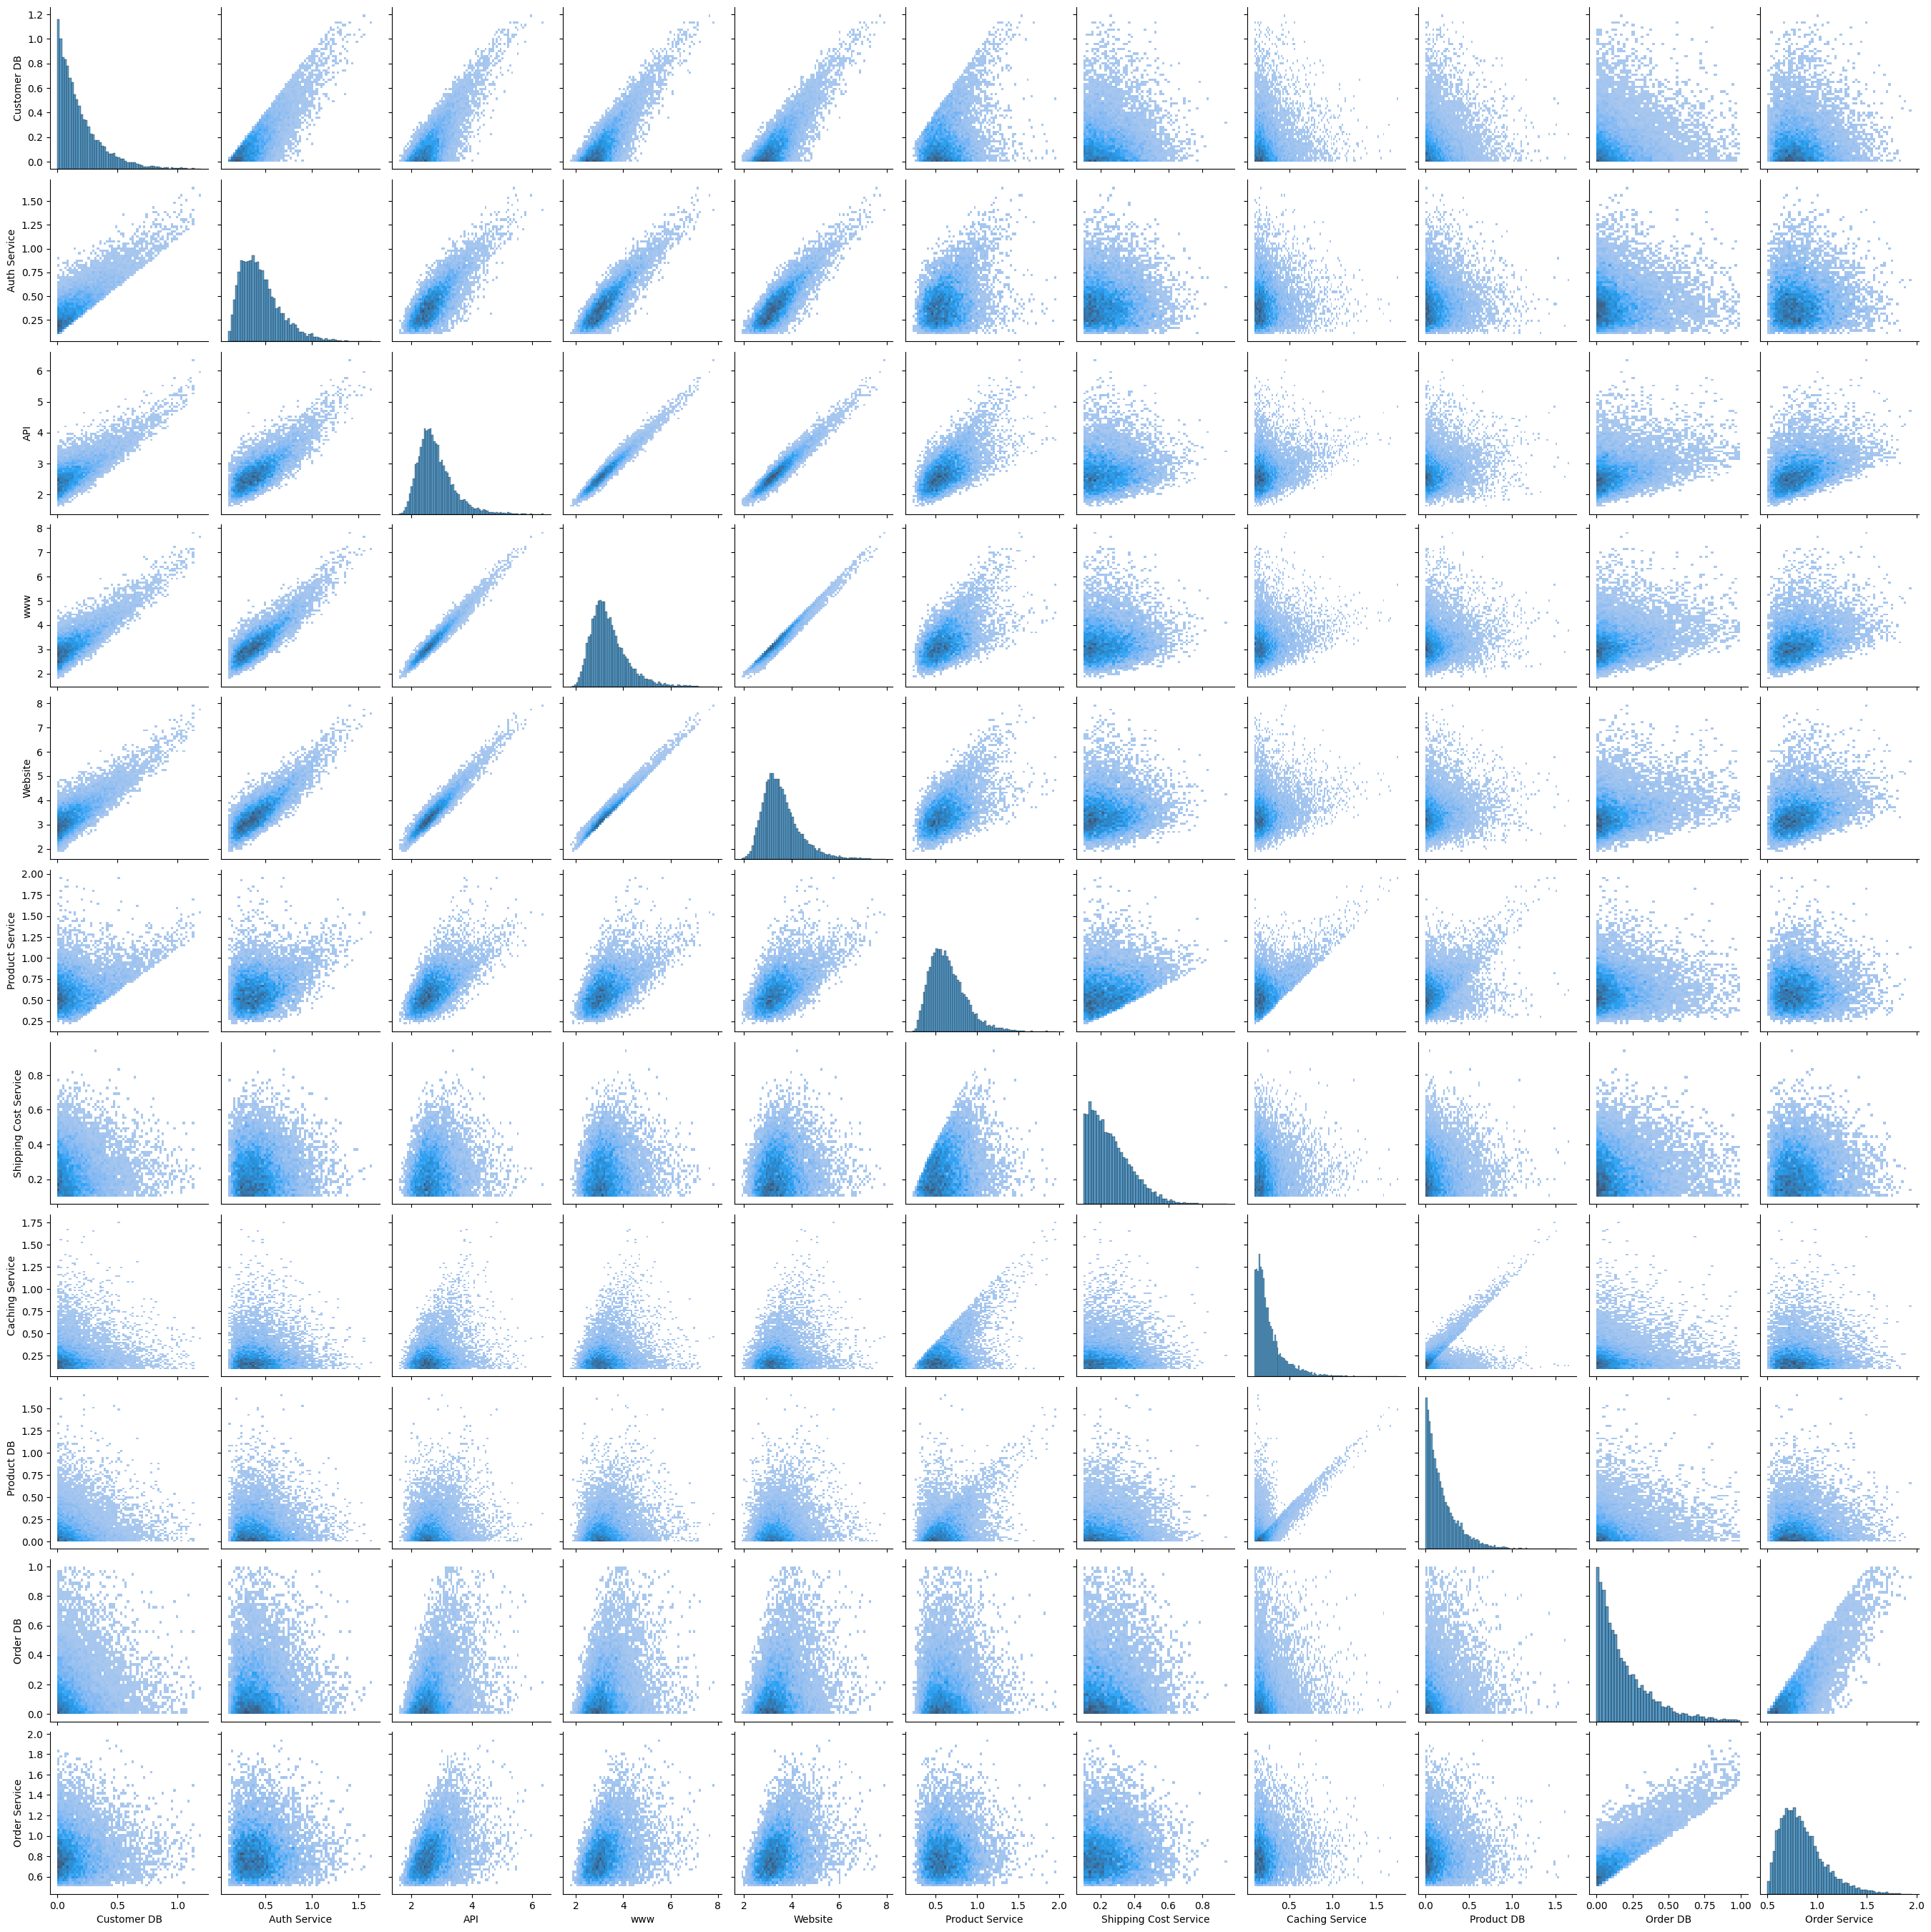
\includegraphics[height=0.8\textheight]{pairplotraw.png}
    \end{center}
\end{frame}

\begin{frame}
    \frametitle{Visualizing with copulas $3$}
    \begin{center}
        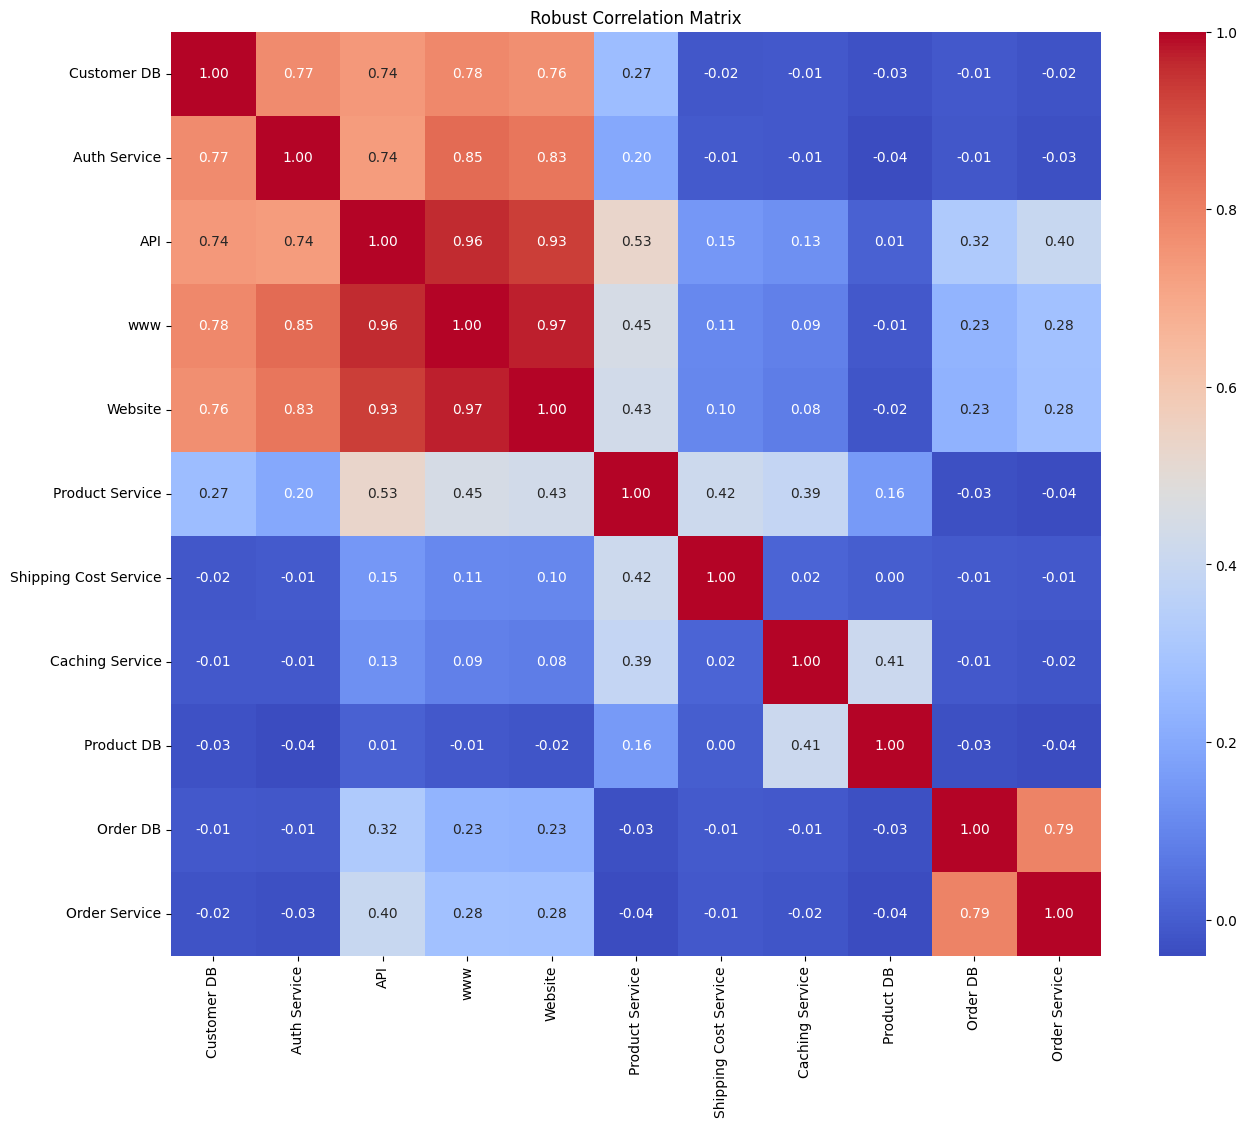
\includegraphics[height=0.8\textheight]{robust_correlation.png}
    \end{center}
\end{frame}

\begin{frame}
    \frametitle{Visualizing with copulas $4$}
    \begin{center}
        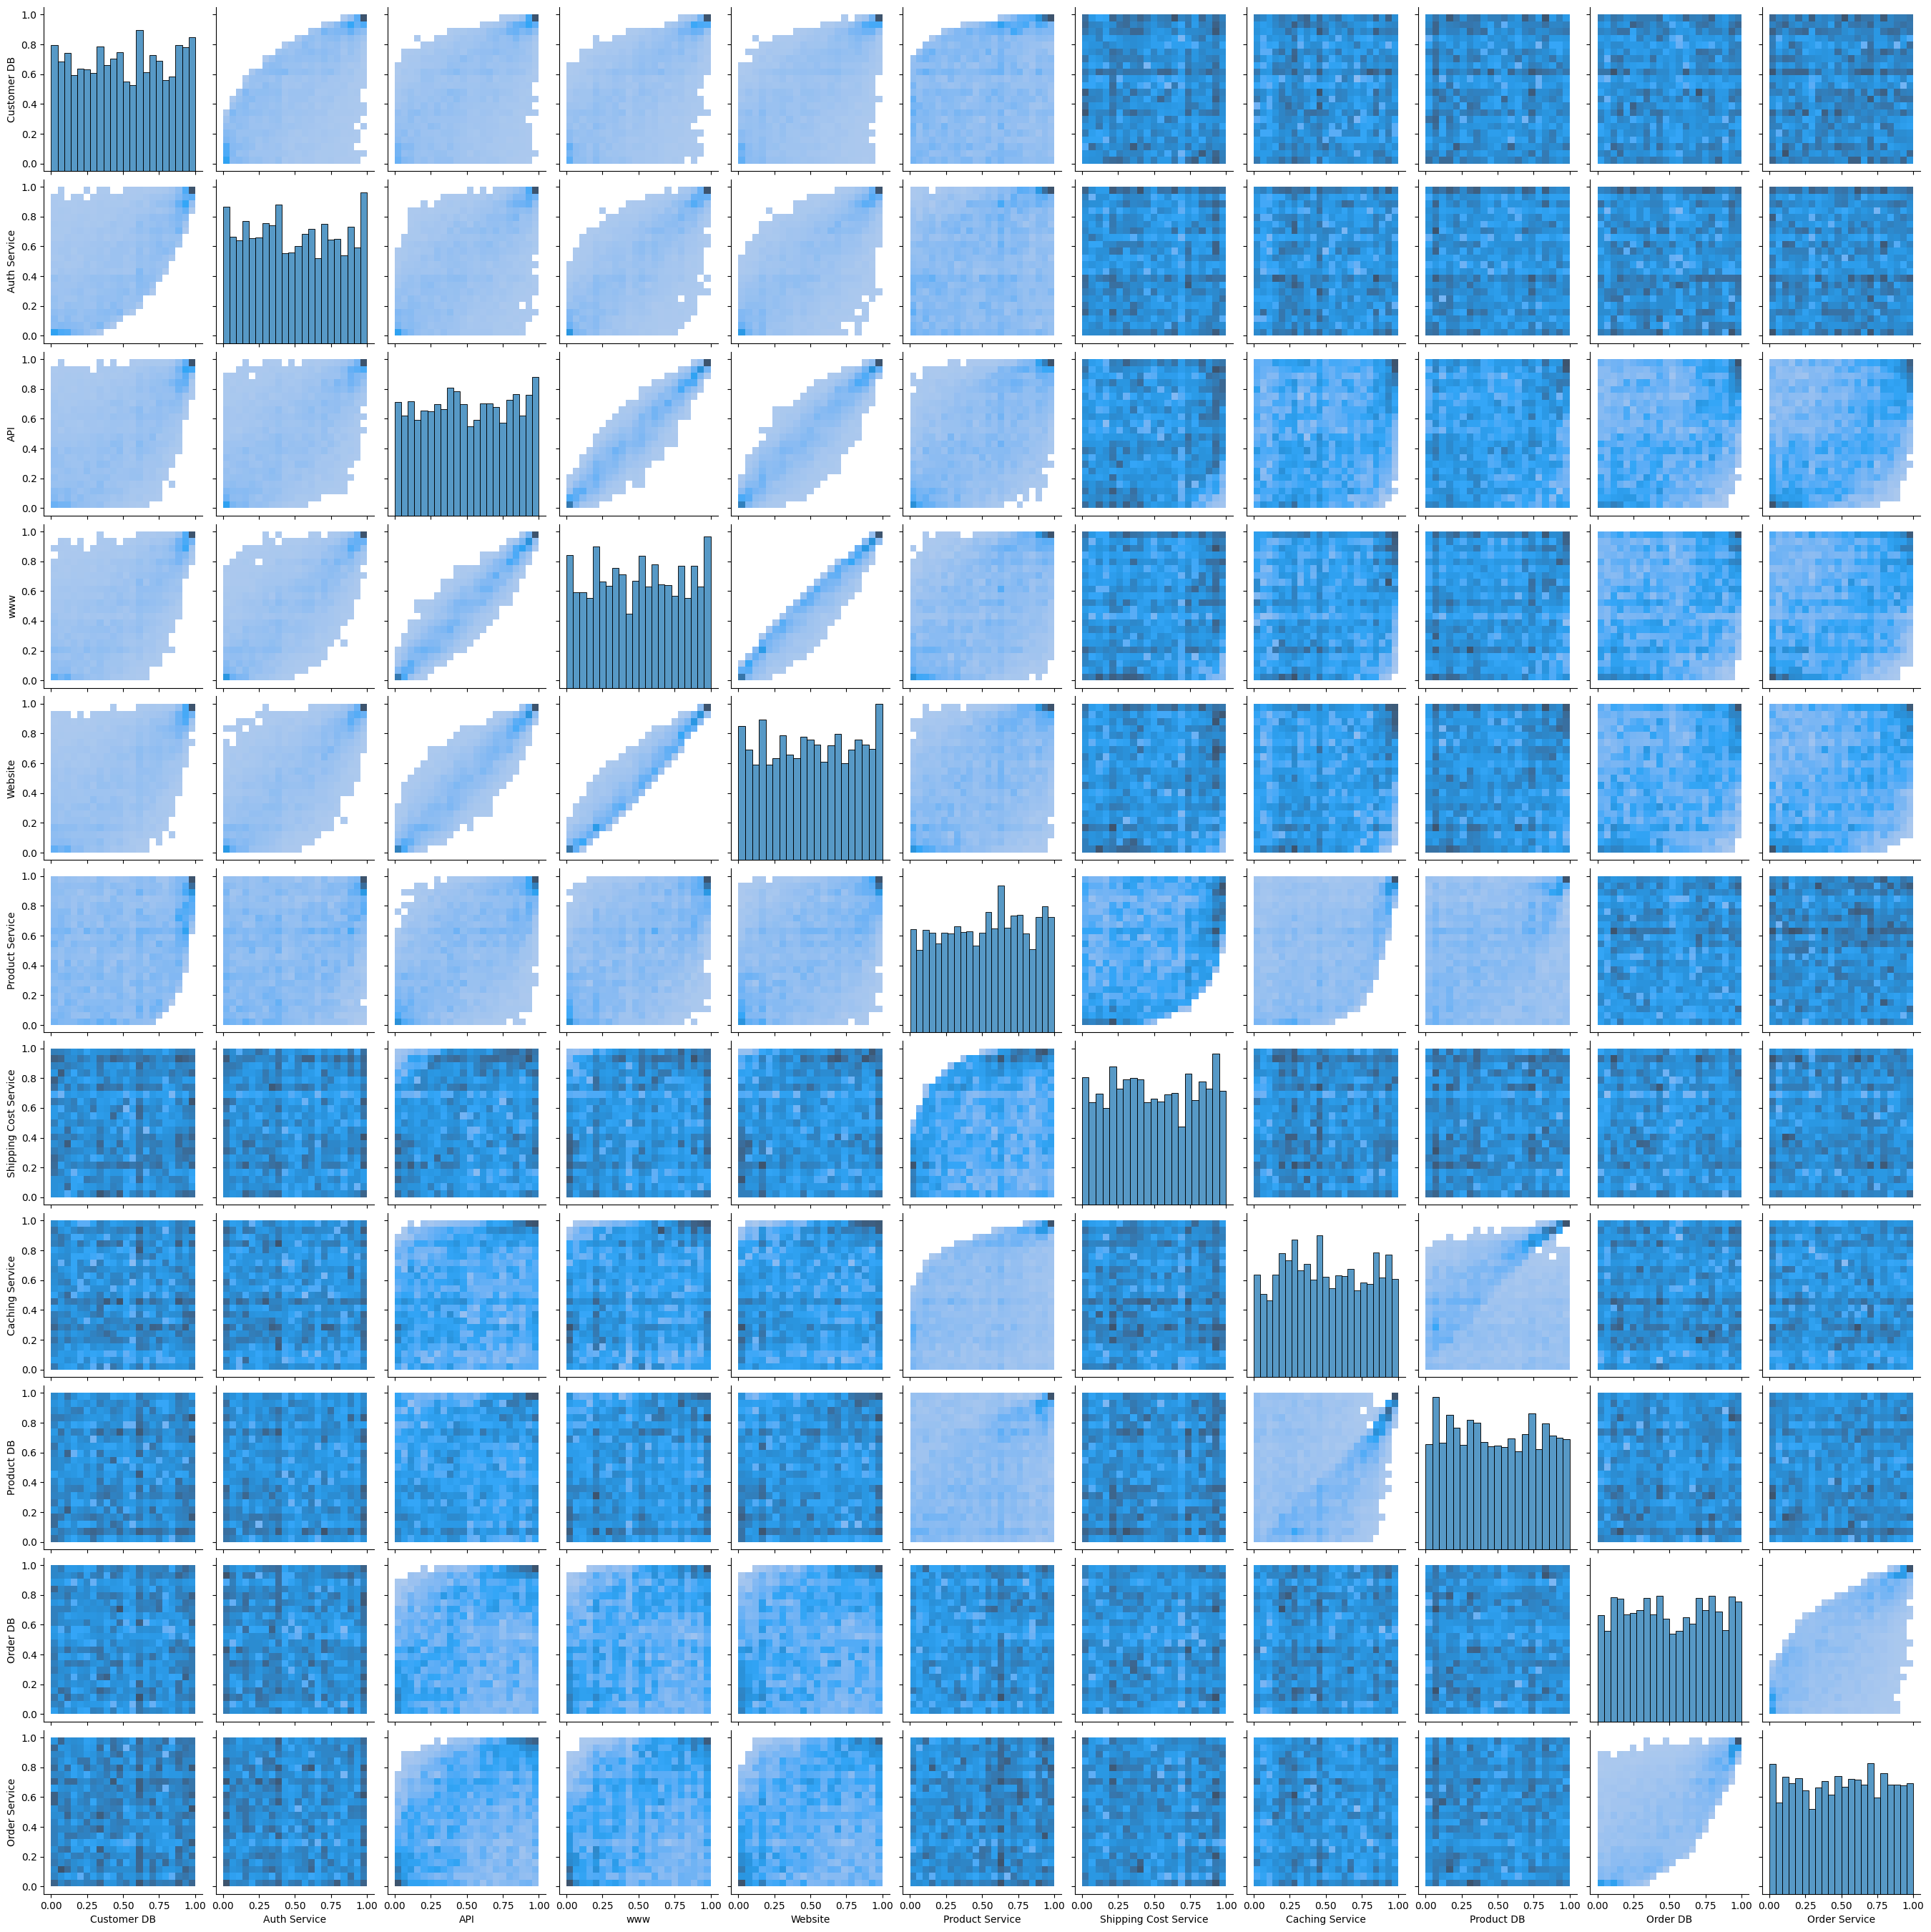
\includegraphics[height=0.8\textheight]{psuedocopulapairplot.png}
    \end{center}
\end{frame}


\begin{frame}
    \frametitle{Copula cons}
    \begin{itemize}
        \item Reliant on parameteric assumptions in high dimensions
        \item Copulas don't always retain smoothness/other properties
        \item Difficulties with multimode distributions
        \item Density estimation (breaking Vapnik's principle)
        \item High dimensional dependence is unintuitive and complicated
    \end{itemize}
\end{frame}



\begin{frame}
    \frametitle{Conclusion}
    \begin{itemize}
        \item Copulas are a powerful tool for modelling dependence
        \item Theoretical tools for understanding dependence
    \end{itemize}
\end{frame}


\end{document}